\documentclass{article}

\usepackage[OT1]{fontenc}
\usepackage{mathpazo}
\usepackage[english]{babel}

\usepackage{amsmath}
\usepackage{amsfonts}
\usepackage[utf8]{inputenc}
\usepackage{graphicx}
\usepackage{float}
\usepackage{hyperref}
\hypersetup{
    colorlinks,
    citecolor=black,
    filecolor=black,
    linkcolor=black,
    urlcolor=black
}

\title{\textbf{Artificial Intelligence}}
\author{Manuel Pagliuca}

\begin{document}

\maketitle
\tableofcontents
\section{Motivation}
Artificial neural networks are information processing systems, whose structure and
operation principles are inspired by the nervous system and the brain of animals and
humans.

Artificial neural networks are studied for various reasons.

\begin{itemize}
    \item Extracting knowledge from data (\textit{phenomena, events, processes, operating environment,...}).
    \item Understanding the phenomena that I’m observing, extracting the knowledge about that phenomena.
    \item Automated construction of computational paradigms for problem solving.
\end{itemize}

The ultimate goal is to be able to have a model which allow to describe the phenomenon
that I’m observing and using this model I would like to solve the specific application problem.

There is an huge variety of application, this is the reason which AI now is so popular, and we
have so many interested and expertise in this field.

The next evolution of the economy is based on availability of solution which are extracted
from the data by analyzing the data reasoning, the only problems is that our capability
of reasoning is limited by the fact that our brain is not able to analyze huge quantity
of data, with automated system we can exploit this and make more comprehensive models that describe
the process of systems we are observing and develop more accurate solutions.

Basically, artificial intelligence is mimicking the nature. We want to take the data
analyze the data make a model, and for doing this we use techniques, we want to enrich
the analysis we are doing through sensors from environments, we can use other
specific sets of techniques.

We have the need of putting together some ideas and observation, we can define rules for reasoning, we extract the knowledge,
but we can also build knowledge through reasoning. Basically, what we want to do is to try to replicate
how the living beings observe and operate in the environment, how express, interacts.

Not only but we want to observe how the individual evolves, population evolves, in order to understand the trend
of the environment. In this broad variety of approaches is to define some techniques which mainly are
in two big categories, from the point of view of intelligence :

\begin{itemize}
    \item \textbf{Symbolic approach}
    \item \textbf{Sub-symbolic approach}, which are sub-symbolic techniques for analyze the environment
          and the systems.
\end{itemize}

During this course we are focusing on sub-symbolic reasoning techniques:
\begin{itemize}
    \item \textbf{Neural networks}, which is a simulation of a living brain.
    \item \textbf{Fuzzy systems}, which embed the definition of quantities, which are fuzzy (not defined
          in a very crisp way).
    \item \textbf{Evolutionary computing}, which is a set of techniques which mimics the natural evolution of the
          species so we can try to optimize the solution by using the basic concept of the natural evolution of the species.
\end{itemize}


\section{Neural networks}
\subsection{Biological background}
Basically, the aim of the artificial neural networks in \textit{mimicking} the behavior of our brain starts
from the fields of neural biology and neural physiology. What this discipline tries to do is to analyze the
behavior of the biological neurons cells and understand how they behave for retrieving
the information from the outer world.

The neurons use sensors and special cells to connect to the external world and get information.
As humans or other biological species, we have five senses, taking for example the eyes, they are receptors
which are able to see what a round us is, they are able to reconstruct the scene we got around us.

Basically, with artificial neural networks we are trying to replicate what \textbf{biology} does for us, in neurobiology
we build a model of what is happening in the neurons, this model describes how the neurons are
interacting together to extract the knowledge, to build memory, construct reasoning, take decisions.

In computer science we want to build this model in computer just for trying to do something similar, we want to mimic the
behavior of the natural brain in order to try to replicate in an artificial environment the same operation.

We are building the \textit{model} for neurons in the computer, in this way we are able to use these
artificial models to \textit{learn} the environment and to solve practical problem (predict possible behaviors
and solve optimization problem, like we do naturally). We also have some basis in other disciplines like
physics and chemistry since we may want to use the neural networks, also for describing physical phenomena,
not only to create reasoning in our mind but we want to create models of phenomena, this can be used for various application.
We can create an abstract model, and instead of observing the real world we can observe how the model behave in some conditions.

Neural networks and in general artificial intelligence, is a discipline of computer science and
engineering, then we use some inspirations from other discipline but the core of the theoretical aspect
of the foundation which defines the artificial neural networks this is an area which is been to computer science and engineering.
\subsection{Reasons for studying the biological background}
The reasons for studying the BB (\textit{biological background}) in computer science are two:
\begin{itemize}
    \item The \textbf{first reason} for studying the neural networks is the fact that they are a very appealing model,
          since they work in \textbf{parallel} means that they have an intrinsically extremely high \textit{parallel process capability}.
          This is why computer scientist are so attracted to this topic. Our brain in many cases find the solution immediately, this
          is fascinating, this happens because we are exploiting the parallel capability of our neural networks.
    \item The \textbf{second reason} why we are studying this technology is the fact that there is really a huge amount of \textit{practical
              application} in broad variety of area : \textit{industrial manufactory, products medicine, finances, economy, social networks, data analysis, ...}
\end{itemize}

\subsection{Neurons}
\begin{figure}[H]
    \centering
    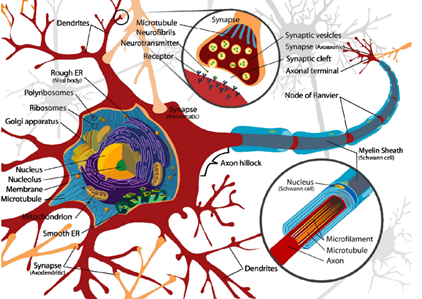
\includegraphics[width=10cm]{images/neuron1.png}
    \caption{Neuron}
    \label{fig:neurone_1}
\end{figure}

The \textit{central} part of the neuron is the part, which is managing the entire cell, this core the
nucleus is listening what is happening around the neuron,
when I have a \textbf{solicitation} from the external (other neurons or special cells related to the five senses).

When there is sufficient stimulation coming from this cells the nucleus is solicited and at a given
point the nucleus realizes that the solicitation is so high that he has to
take an \textbf{action}, the action is to send a \textit{signal} around the \textit{axon} (the long extension covered in blue),
this will lead to have a \textit{polarization} of an \textit{electric signal} which is flowing along this connection
and this will reach other neurons that are connected to the end of the axon to the synapses.

\begin{figure}[H]
    \centering
    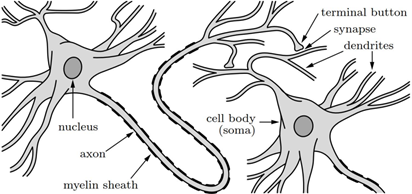
\includegraphics[width=10cm]{images/neuron2.png}
    \caption{Connection between two neurons}
    \label{fig:neurone_2}
\end{figure}

The \textbf{axon} is covered by an appropriate \textit{protein} (covered in blue) which protect the axon itself,
and make sure that the polarization that occur on the nucleus is transmitted along the axon so that this signal is able
to reach the synapse.

Basically, what we see is that the \textbf{neuron is exciting the nucleus}, which is generating the excitation along the axon,
then it will reach the terminal synapses.

Each synapse is connected to the synapses of \textit{another} neuron, so that the signals which are generated by
the nucleus and sent to the axon and then to the synapsis terminal at the terminal the synapses
are releasing some chemicals called \textbf{neurotransmitters}.

These \textit{substances} are exciting the synapses of the connected neuron, bu stimulating the synapses this excitation is
propagated from the \textbf{dendrites} to the nucleus of the other neuron, when the other cell is \textit{sufficiently excited} by
from the amount of stimulation generated by the neurotransmitter the nucleus will generate again a new stimulation
which is going along the axon and reach another neuron (and so on...).

The axon is \textit{depolarized} if there is enough excitatory input, basically this is how the signals are propagated
through the brain.

Due to the fact that each neuron can stimulate each other neurons connected to them,
this will create the \textbf{parallel processing} in our brain, so that each component will take care
of analyzing each part of the information and this is a consequence to derive a part of the total computation.

\subsection{Computer vs Human brain}
When we look to the differences between a computer and the human brain what we notice,
is that in the computer we got processors composed by many \textit{transistors}, the human brain counterpart
the got $10^11$ \textit{neurons}, the number of the latter overcomes the number of the cores in a processor.

The neurons aren’t able to process the same \textit{complex operation} of a core, but they are still so many that they
can overcome the limit of the complexity of the individual operation with the fact that they are working significantly in
parallel.

\begin{figure}[H]
    \centering
    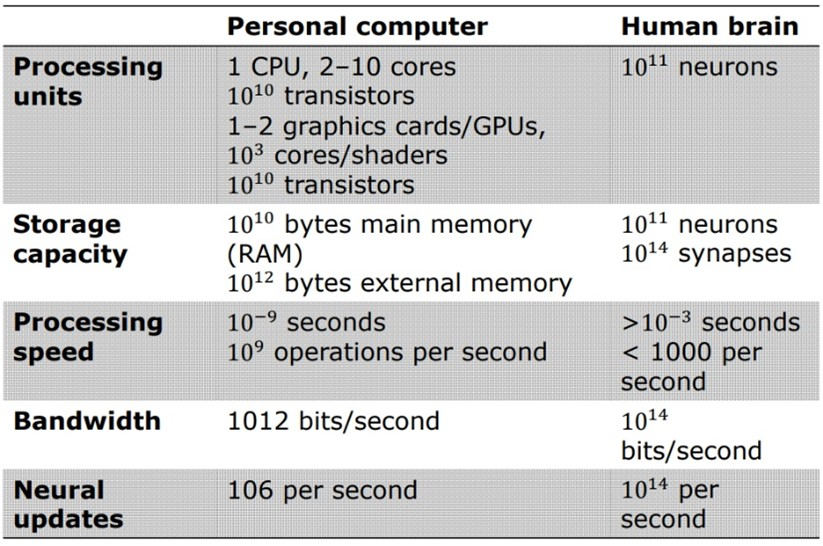
\includegraphics[width=10cm]{images/tab_pc_vs_brain.jpg}
    \caption{PC vs Human brain}
    \label{fig:tab_pc_vs_brain}
\end{figure}

The \textbf{storage} of the neurons has an immense storage potential than any other memory capacity. The \textbf{processing speed}
seems \textit{much higher} on the computer, but the parallel operation that you can do in parallel in the human brain in
the end \textit{overcome} the processing speed of the hardware of a computer.

Basically, what we can observe is that the biological neural networks are able to outperform significantly the processor that
we have nowadays, there are some researches carried out which are trying to create processors which are replicating in
hardware the operation of the biological neural networks but still the capabilities of this systems are \textit{far} from the
capability of human brain.

It may \textit{seem} in some system that they are working faster then humans, it may seem that they are running better, but actually
what you have is that you have the ability in the computer to run the algorithms and the explore the
possible (deterministic) moves in a fast way but needs some background knowledge
in order to that in a very short time.

Advantages of biological neural network:
\begin{itemize}
    \item High processing speed due to massive parallelism.

    \item Even if we have a significant amount of the biological neural network damaged, the system is
          considered \textbf{fault tolerance}, it remains functional even if larger parts of the network get \textit{damaged} (maybe some functions will be disabled).
          The other cells are able to overcome the death cells, this thanks to the elasticity of the neurons which are able
          to overcome possible damages in the structures.

    \item If more neurons are failing, the brain will \textit{degrade the performances} in a \textit{graceful way},
          it will not just stop working, will work a bit less not with the same performance and the same functionality
          but with reduced function. Only when a \textit{really massive} number of neurons is dying at that point a
          function is not working anymore.

    \item They are well suited for inductive learning (\textit{learning from examples, generalization from instances}).
\end{itemize}

What we are trying to do with artificial neural networks is to capture the parallel operation of the brain. The ability to
extract the knowledge from the data, we want to replicate these capabilities.

There are some problems due to the \textbf{ANN} (artificial neural networks), if we kill part of the architecture which
is replicating the \textbf{BNN} (biological neural networks), the ANN is \textbf{not automated to survives}, we have to
assure some physical redundance, this is a problem of the architecture we are using to execute the computation of the ANN.

What we want to do in our model is to construct a \textit{set of abstract models of the neurons} that we call
\textbf{artificial neurons}, and we like to connect them together to replicate the structure that we have in the
natural brain this is why we have the ANN, a connection of neurons that is trying to mimic the behavior of the brain.

The complexity of the brain is so high that is actually difficult to replicate everything in ANN,
what we are doing is to replicate a specific function of the brain which is able to solve a specific application
problem that we have.

\subsection{Threshold Logic Units}
This is the first \textit{abstract model} for an artificial neuron of the brain.
A \textbf{threshold logic unit} (TLU) is a \textit{processing unit} (neuron) with several inputs.
It can solve a very simple set of problems.

We have a \textbf{core} (the neuron) with several \textit{inputs} that are reaching the neuron, and we have the
\textit{output} which is delivered to the subsequential neurons which are connected with it.
A TLU is a processing unit in which the output is governed by a threshold $\theta$, if it has a \textit{sufficient excitation}
from the inputs, then the TLU became \textbf{active} (value $1$) and generates the output $y$.

\begin{figure}[H]
    \centering
    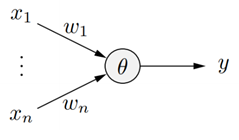
\includegraphics[width=6cm]{images/tlu.png}
    \caption{Threshold logic unit}
    \label{fig:tlu}
\end{figure}

We have $n$ inputs identified by $x_1,…,x_n$ the unit is generating only one output $y$ each input is \textbf{not}
delivered directly to the core of the TLU, but each input is \textbf{weighted}, some are more relevant,
and others are less relevant (exactly how we are doing when we consider the data from the external world).

\begin{figure}[H]
    \centering
    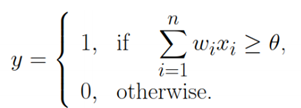
\includegraphics[width=6cm]{images/tlu_working_system.png}
    \caption{TLU conditions}
    \label{fig:tlu_conditions}
\end{figure}

This means that our problem is depending on the most important information, this is what happens in the real world.

In the ANN we are replicating the relevance of the individual input, we can control how much each input is actually
important to influence the generation of the output, to do this we use a weight $w$ for each of the input so
that the TLU will not see exactly the input but will see a weighted input, this will allow the modulation of
each input by giving to each of them the appropriate importance during the generation of the final output.

When the TLU is solicited enough it will generate an output $y$ that will be delivered to the \textit{terminal synapse}
to another neuron.
\begin{itemize}
    \item If the \textbf{excitation is enough}, mathematically means that the weighted summation is greater
          than a thresh $\theta$, we generate $1$ (the neuron is active).
    \item If the \textbf{excitation is not enough} for overcoming the threshold $\theta$, we generate $0$.
\end{itemize}

This model that tries to represent what is happening in the BNN from two scientists, also called the \textbf{McCulloch-Pitts neuron}.
\subsubsection{Conjunction example}
The result is equal to $1$ only when the two outputs are equal to $1$.
There is not a standard way to select the threshold $\theta$, we have to choose that in base of the
function that we want to implement. In this case I have to select a $\theta$ which is greater than the biggest weight.

$$x_1\land x_2$$

\begin{figure}[H]
    \centering
    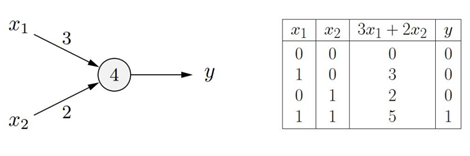
\includegraphics[width=10cm]{images/conj_TLU.png}
    \caption{Conjunction TLU}
    \label{fig:tlu_conjunction}
\end{figure}

\subsubsection{Implication example}
I can choose the value of the threshold in order to have the proper function, in this case applies on the same ways.
\textit{How can I choose the interconnection weights?}

The problem is that there are no general rules, I choose the weights according to the intrinsic relevance of each
input variable.

\textit{How can I do that when we have a high number of inputs?} we will see that there is a procedure for doing that.
$$x_2\rightarrow x_1$$
\begin{figure}[H]
    \centering
    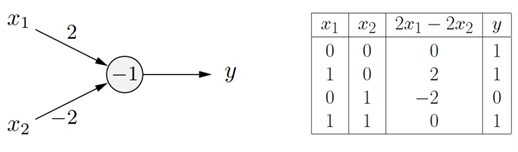
\includegraphics[width=10cm]{images/impl_TLU.png}
    \caption{Implication TLU}
    \label{fig:tlu_implication}
\end{figure}

\subsubsection{Multiple inputs example}
In this case we can see that we have three possible inputs, we can discriminate the
inputs in excitatory input and inhibitory input. The first tries to contributes
to the final computation of the neuron in such a way that the results
will be greater than the threshold, the other neuron does the opposite.

\begin{figure}[H]
    \centering
    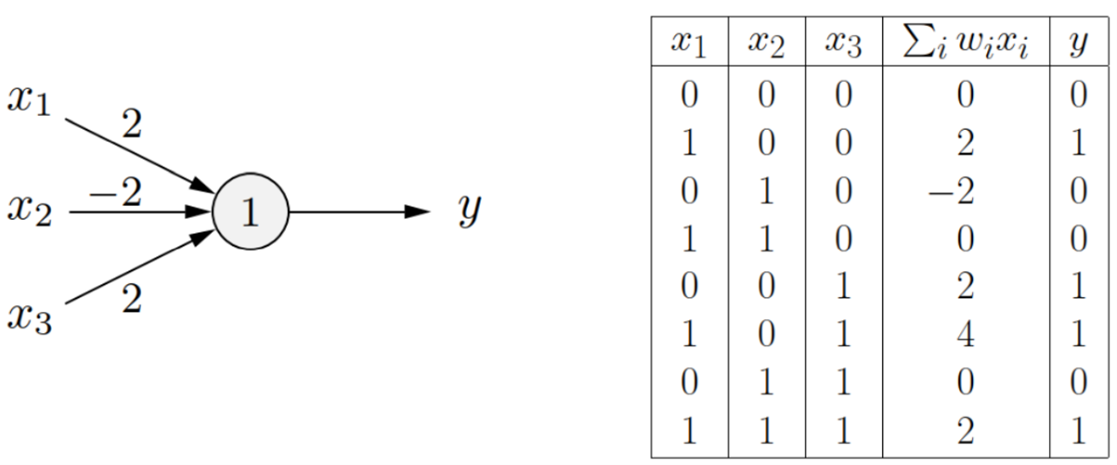
\includegraphics[width=10cm]{images/complex_TLU.png}
    \caption{Three-input TLU}
    \label{fig:tlu_3_input}
\end{figure}

\subsection{Geometric interpretation}
The geometric interpretation is significantly helpful to derive a \textit{method} to
configure the threshold and the weights starting from the data. We will consider a
single and simple TLU, we will try to understand how we can interpret the
behavior of the TLU in a geometrical way.

You know that is possible to represent a straight line on a plane in any of
the following forms :
\begin{figure}[H]
    \centering
    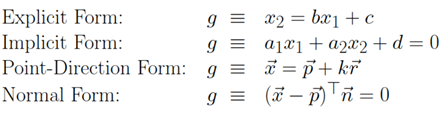
\includegraphics[width=10cm]{images/geom_interp.png}
    \caption{Different form for representing a straight line}
    \label{fig:line_repr}
\end{figure}

If i \textbf{implicit form}, where you have a weighted combination of the two variables plus a
possible threshold, a vector representation in point-direction form and normal form.
Any of this is fine to represent a straight line in the plane, we are considering just
two variables $x_1$ and $x_2$, and use one of the many representations.

\begin{figure}[H]
    \centering
    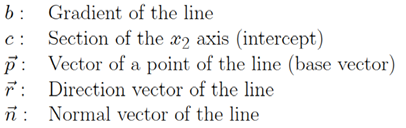
\includegraphics[width=9cm]{images/geom_interp_impl.png}
    \caption{Implicit form representation legend}
    \label{fig:line_impl_form_legend}
\end{figure}

\begin{figure}[H]
    \centering
    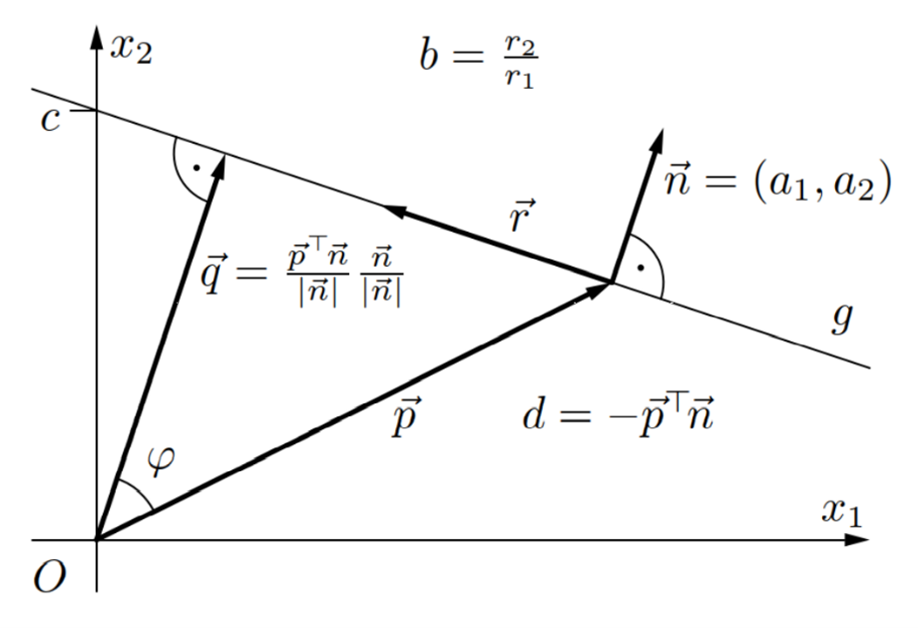
\includegraphics[scale=1]{images/geom1.png}
    \label{fig:geom_1}
\end{figure}

In the case of the \textit{explicit/implicit form} the $\vec{b}$ is the \textbf{inclination}
(or \textit{gradient}) of the straight line in respect of the horizontal axis,
and $c$ is the intercept of the vertical axis.

If we look to the normal $\vec{n}$ we want to pick the vector which is \textit{orthogonal}
to the straight line. The straight line is represented by all the points which starts from the
origin and has a quantity in the direction of the normal. The vector $\vec{p}$ identifies a
point in the example, we consider that point belonging to our straight line,
the distance of the straight line respect to the origin $O$ is given by $|\vec{q}|$ which is
the projection of $\vec{p}$ on straight line $g$.

\begin{figure}[H]
    \centering
    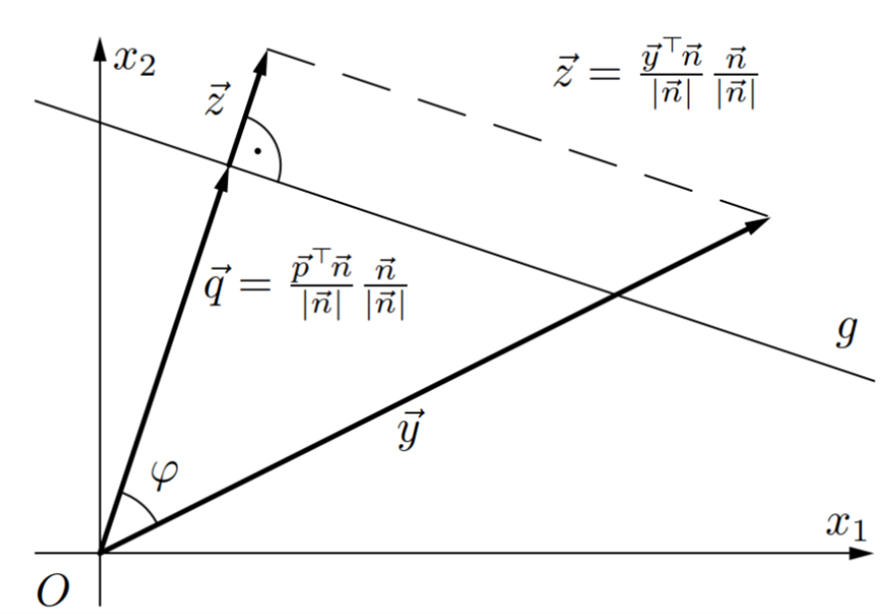
\includegraphics[scale=1]{images/geom2.png}
    \label{fig:geom_2}
\end{figure}

Considering this other graphical representation it is possible to know on which side
a points lands. If we take the vector representing $\vec{y}$ a point,
and i compute the projection in the direction of the normal, the projection
of this is the vector $\vec{z}$.

To understand on which side the points are, i just need to see if the vector $\vec{z}$ (which is the
projection of our point) is shorter or longer than the point i observe on the straight line, which
is pointed by $\vec{q}$. This means that all points (expressed by a vector) which have a \textbf{module}
higher then the projected point onto the straight line ($\vec{q}$), are part of the plane above the
straight line (they will \textit{satisfies} the solution), viceversa, they will be below the plane if the
module will be shorter then $\vec{q}$ (they won't satisfy the condition).

Basically the straight line which defines the behavior of my TLU, splits the plane in two parts (since i'm
considering only $x_1$ and $x_2$). All the points which distance is greater then

\begin{figure}[H]
    \centering
    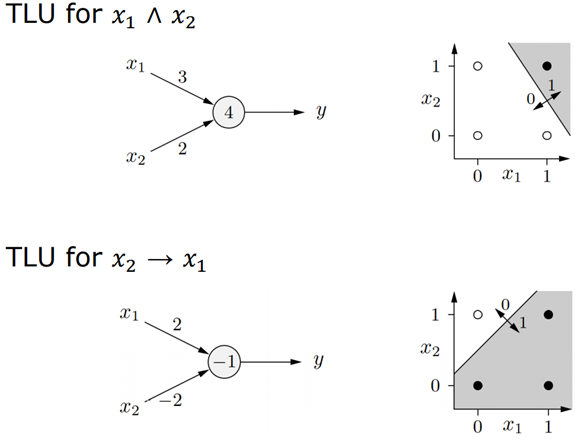
\includegraphics[scale=0.8]{images/tlu_examples_interp.png}
    \caption{Solution of the \textit{conjunction} and \textit{bi-implication}}
    \label{fig:example_interp}
\end{figure}

Now Let’s go back to the two examples that we have seen before,
starting with the conjunction, in this means that I have three points in which the output
has to be $0$, and one point where the result is $1$. This means that if I represent the straight
line with $x_1=3$, $x_2=3$ and the intercept equal to $4$ i will draw a line which is actually
separating in a clear way the element in which the output is equal to $1$ from the values
where the output is equal to $0$.
\newline
\newline
For the case of three variables, this is more complex, we need to generalize this idea moving from
a plane to a three-dimensional space. Think about the three axis and look at the combination of the
dots, you need to set a plane, so you have to separate one set of inputs for which the output has
to be equal to $1$ from the set of inputs combinations where the output is equal to $0$.

\begin{figure}[H]
    \centering
    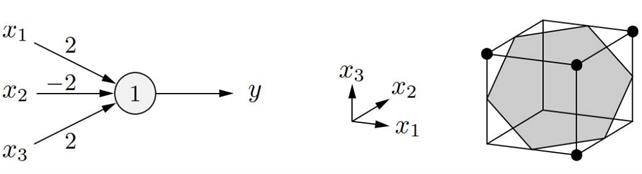
\includegraphics[scale=0.6]{images/three_input_sol_example.png}
    \caption{Solution of the complex TLU}
    \label{fig:example_three_sol}
\end{figure}

Basically, if you represent the plane using these information’s you will have this
kind of plane (that looks like a hexagon) dividing the solution from the $0$ values.

\textit{So how we choose the threshold and interconnection weights?} I have to look at geometrical
distribution of the points for the combination of the input which the output must be equal to $1$
and the one where the output must be equal to $0$, I have to take a straight line or plane and I
need to position the divisor in a way that I clearly separate the two groups. If I can do that,
that set of values (inputs and threshold) are the one that I need to use in my ANN.

\begin{figure}[H]
    \centering
    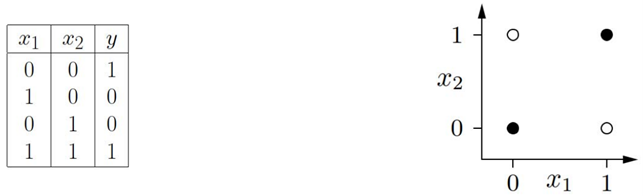
\includegraphics[scale=0.6]{images/bi_implic_no_sol.png}
    \caption{The bi-implication problem}
    \label{fig:bi-impl-problem}
\end{figure}

Let’s analyze another example, the bi-implication problem, this problem results in this kind of
distribution in the plane, as you can see it is not possible to separate these points with a
straight line. As a consequence, we don’t have any TLU for solving this problem, even if this is
a simple problem. We have to introduce some notions for understanding the reasons behind
this problem.
\subsubsection{Linear separability}
Two set of points in the \textbf{Euclidean Space}, consider $x_1, x_2,...,x_n$ as the variable for
the TLU, since we have n possible inputs you are analyzing a problem represented in $n$
dimensional Euclidean space.

If you have in this Euclidean space two set of points they are \textbf{linearly separable},
if and only if there exists at least one point, line, plane or hyperplane, such that all
points of the first set lie on one side and all points of the other set lie on the
other side of this point, line, plane or hyperplane.

The point sets can be separated by a linear decision function.

If you are in a mono dimensional space you have one input only,
your Euclidean Space is a line, you have one point on this straight line which is separating
your space the line in two parts, the output is one, for the other point the output is $0$.
If you have a plane, we have two input variables, we have to find a plane that separates
the two sets of points.
\subsubsection{Convex hull}
A set of points in the Euclidean Space is called \textbf{convex} if it is non-empty and
connected and for every pair of points in it every point on the straight-line segment
connecting the points of the pair is also in the set.

A \textbf{convex hull} of a set of points $X$ in a Euclidean Space is the smallest convex set of
points that contains $X$. Alternatively, the convex hull of a set of points $X$ is the intersection
of all convex sets that contain $X$.
\subsection{Solution of the bi-implication problem}
Two sets of points in Euclidean Space are linearly separable if and only if their convex hulls
are disjoint. In the bi-implication problem, the convex hulls are the diagonal line segments.

They share their intersection point and this means that they are not disjoint, therefore
the double implication is not linearly separable.

\begin{figure}[H]
    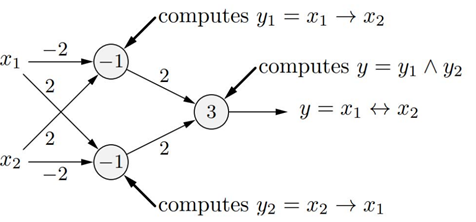
\includegraphics[scale=0.8]{images/sol_bi_implic_problem.png}
    \centering
    \caption{TLUs to the bi-implication problem}
\end{figure}
What we can do is putting together more neurons to try to address more complex problem where
one neuron can’t solve. We are creating a network of TLUs, we are splitting the problem in two
sub problems.

The problem of implication can be solved with a single TLU, we create a more complex structure
in which are able to solve the problem.

Let’s see what happens geometrically, the two points $a$ and $c$, are going to be separated
from the first two  TLUs, I set one of the TLU so that all points which are below the straight
line represented by $g_2$ fives and output equal to $1$, and then i set a second straight line
represented by $g_1$ where all points are all over the straight line the values are equal to $1$,
and then I merge this information.

\begin{figure}[H]
    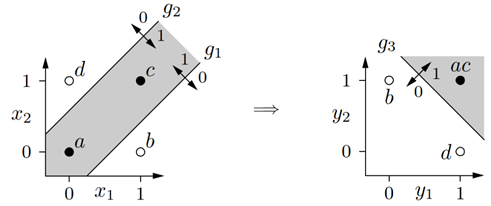
\includegraphics[scale=0.8]{images/sol_bi_implic_problem_graph.png}
    \centering
    \caption{Solution of the bi-implication problem}
\end{figure}

I combine these information from the previous group in the third neuron so that I transform
the representation of the information, I can merge the information of the points $a$ and $c$,
so that both the output of the two TLU is equal to $1$ is represented by one points (in this case
they are the same) and then I have the two other points $b$ and $d$ which are in both the parts
above and below the line, for them the solicitation is not enough to generate an output
equal to $1$, as a consequence I obtained a linear separability.

I transformed the stripe in a semi plane with the third TLU, which identifies the linear
separability, I don’t have that propriety only with the first TLU but also with the second,
both TLUs allow me to partition the first space in three parts.

\subsection{Arbitrary boolean functions}
I can work with any arbitrary \textbf{Boolean function}; in this example I have a
Boolean function of three variables. I have these values of the value $y$ according to the formula.

\begin{figure}[H]
    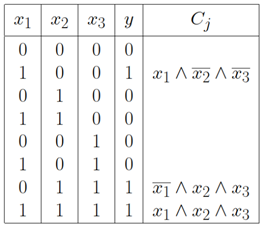
\includegraphics[scale=1.0]{images/arb_bool_funcs.png}
    \centering
    \caption{Table of values}
\end{figure}

What we can do is to build a network of TLUs that allow me to compute each of the component
for which the output has to be $1$ and then with a conjunction unit I put together all
the possible value with a or for merging the individual TLUs.

\begin{figure}[H]
    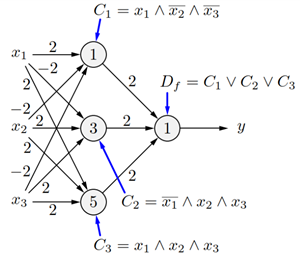
\includegraphics[scale=1]{images/arb_bool_funcs_graph.png}
    \centering
    \caption{Network of TLUs solving the boolean function}
\end{figure}


\subsection{Training TLUs}
The geometric interpretation that we have seen before about the operation of TLUs gives us the
understanding of how we can place the various parameters for our networks in order to
construct TLUs with $2$ and $3$ inputs.

But this makes sense when we are using $2$ or $3$ input, but this is something that is not
feasible when we are having more than three inputs, also this is not an automated method.

We want an automatic method for visualizing the space and points in the space, especially when
we have more then $3$ inputs.

What we want to do is to have an automatic way which adjusts the weights and the threshold
of the network so that I can reach the desired solution (if the two sets are linearly separable).

The \textbf{automatic training} of TLUs consist in the fact that we can start from a random value
of the weights and threshold, and then when we want to configure a TLU we need to evaluate
the error that we are generating at the output (of the TLU) in respect to the input pattern
that we have presented.

Basically, we have chosen randomly the threshold, the TLU generates an output, we evaluate
the error respect to the desired output, and then we try to adjust the weights and the
threshold to reduce the error.

We repeat this operation for all inputs until the error is really reduced or vanished.
\begin{enumerate}
    \item Start with random values for weights and threshold.
    \item Determine the error from the output of the TLU.
    \item Consider the error as a function of the weights and the threshold $e=e(w_1,...,w_n,\theta)$.
    \item Adapt weights and threshold so that the error becomes smaller.
    \item Iterate adaptation until the error vanishes.
\end{enumerate}

\subsubsection{Negation example}
\begin{figure}[H]
    \centering
    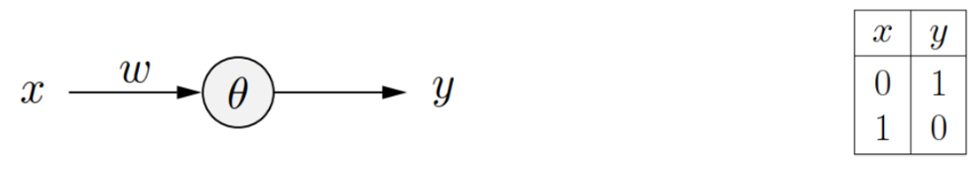
\includegraphics[scale=1]{images/neg_example.png}
    \caption{TLU that perform negation}
    \label{fig:neg_example}
\end{figure}
$$\neg x$$
In this case we have two really simple parameters, the weights and the threshold.
Let’s represent the error for all possible weights and all possible threshold at least
for a subset that we are interested in analyzing. Let’s consider the $x=0$, in this case
the desired output is $1$, if we take $w=2$ and we multiply it by $0$ the weighted input
will be $0$.

\begin{figure}[H]
    \centering
    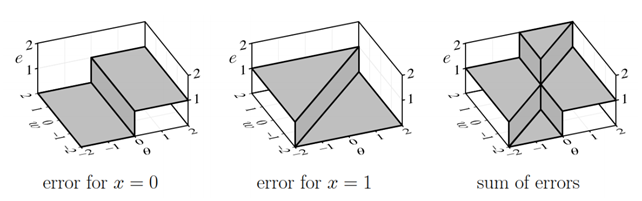
\includegraphics[scale=0.7]{images/errors_exampl.png}
    \caption{Diagrams of the errors expressed in terms of $\theta$ and $w$}
    \label{fig:neg_tlu_errors}
\end{figure}
Let's consider the first diagram on the left, with the various values of $\theta$ and $w$, and
with an input value of $x=0$.
Let's see the error that we have with the various possible combinations, we see that
for any values of the weight where the threshold is \textit{less} than zero, the \textbf{error}
is zero. Viceversa, for any value of the weight for a $\theta$ greater or equal to zero, the
error is one (a \textit{plateau}).

Now let's consider $x=1$, we are on the central diagram, in the left triangular part
of the domain there will be the error of $1$ defined $\forall w$.

Let's try to sum the errors and see what we obtains: we get an intersection for the error
equal to one, and also an intersection for the error equal to \textit{two} (which is strange,
since the error in this kind of example is always $1$ since the $y$ output is binary, but there
we are talking about a sum).

The only part where the error is equal to zero is a small triangle on the bottom. The problem
with this definition of the error is that is not suited for define an algorithm which allow
me to find the zero error.

\begin{figure}[H]
    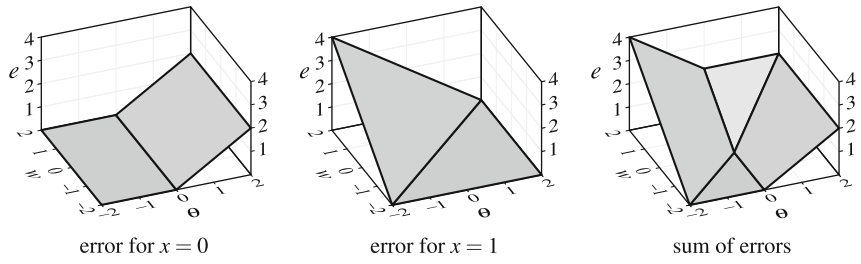
\includegraphics[scale=0.6]{images/desc_2_of_error.png}
    \centering
    \caption{Output error modified as function of weight and threshold}
\end{figure}

What i can do is modify the description of the error and consider that for each value
of the input i will not have just the error which is $1,0$ or $2$, but i will consider
a covering and continuos \textbf{surface area} (such that is possible to increase progressively
the error).


\subsection{Artificial neural network}

\end{document}